\begin{newpage}
  \section{Develop}
  \label{sec:develop}
    % TODO: AWS - Instanz spezifikationen (Leistung) Medium Instanz?
    % TODO: AWS - Server Test bzw Metriken?

    In dieser Arbeit wird ein Macbook Pro 2,9 GHz Intel Core i5 mit 16 GB 1867 MHz DDR3 und Intel Iris Graphics 6100 1536 MB eingesetzt.
    Für das Backend wird die Datenbank PostgreSQL und Nodejs verwendet. Nodejs ist nicht nur einfach aufzusetzen, sondern auch sehr performant und effizient für Web Applikationen einsetzbar. Zudem lässt es sich sehr einfach mittels Docker in der AWS (Amazon Web Services) Cloud veröffentlichen.\\

    Dieses Kapitel ist in zwei Abschnitte unterteilt. Namentlich \texttt{Backend} und \texttt{Frontend} genannt. Im Abschnitt Backend sollen die Implementierungsschritte für das Erstellen eines Backends beschrieben werden, dass ein GTFS-Feed verarbeiten und dessen Daten dem Frontend zur Verfügung stellt. Der Abschnitt Frontend beschreibt verschiedene Performance optimierungen und die einzelnen UI-Komponente mit deren Funktionensweise.\\

    Zu beginn stellte sich die Frage, wie sich in kleinen Schritten an das komplexe Thema einer Live Visualisierung rangetastet werden kann. Die erste Hürde die zu nehmen ist, stellt die Animation vor nur \textbf{einem} Vehicle entlang der Polyline dar.
    Um eine Datengrundlage zu haben wurde ein möglichst vollständiges GTFS-Feed aus \texttt{TransitFeeds.com} ausgewählt und in die Datenbank importiert. Die Wahl fiel dabei auf das Boston-MBTA Feed. Die Herausforderung bestand nun darin, erste Daten aus der Datenbank an den Client zu senden und sie dort darzustellen. Dafür wurde versucht eine möglichst einfache Datenbankabfrage zu finden. Fast trivial ist das abfragen der Polyline: \colorbox{lightGrey}{\texttt{\color{white}{{\color{materialBlue} SELECT} * {\color{materialBlue}FROM} gtfs\_shapes {\color{materialBlue}WHERE} shape\_id = {\color{materialRed}12345}}}}
    Diese Daten werden als GeoJSON übertragen und lassen sich mit Mapbox-gl-js sehr einfach anzeigen. In der Karte ergibt sich daraus eine Route auf der sich ein Vehicle entlangbewegen kann.

    \begin{figure}[htbp]
      \begin{center}
        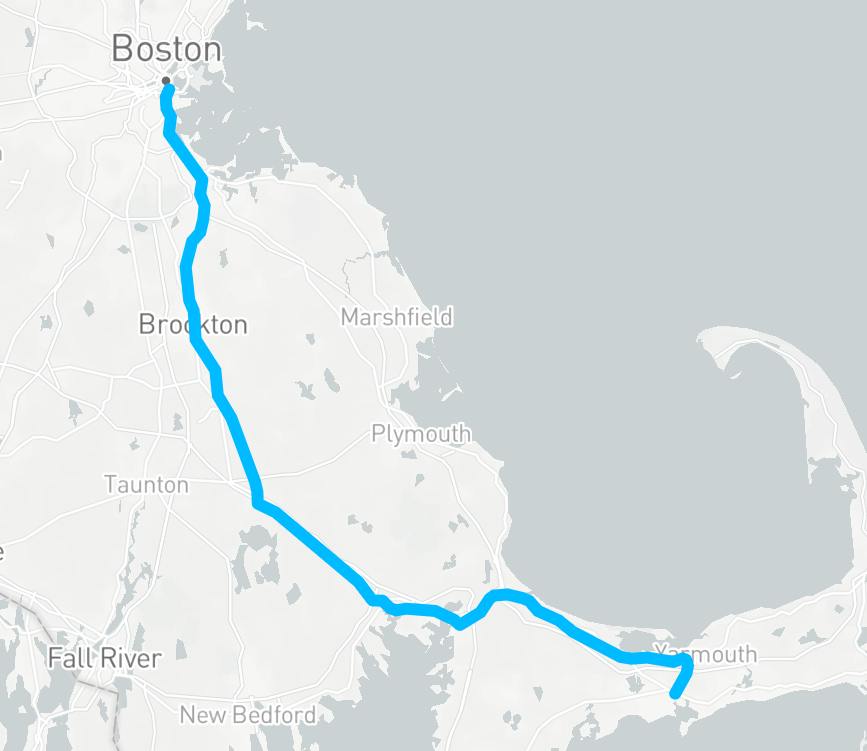
\includegraphics[width=0.5\textwidth]{prozess/draw_single_shape}
        \caption{Anzeigen einer einzigen Polyline in Boston}
        \label{fig:prozess/draw_single_shape}
      \end{center}
    \end{figure}
    
    Abbildung \ref{fig:prozess/draw_single_shape} zeigt das Ergebnis dieser ersten Iteration. Zu sehen ist bereits die Karte und eine blaue Polyline. Nachdem dieser Datensatz auf Client-Seite verarbeitet werden kann, musste das Backend wieder neue Abfragen von Daten ermöglichen. Dieser ständige Wechsel zwischen der Arbeit an Frontend und Backend zog sich durch das gesamte Projekt hinweg durch und stellte sich als sehr effektiv heraus. Erst durch die Arbeit am Frontend, wurde immer wieder klar, welche Daten überhaupt gebraucht und in welchem Format diese am besten sein müssen.\\

    Nachdem die Polyline auf die Karte gebracht wurde, machte es Sinn auch die einzelnen Stationen darzustellen. Damit die Daten besser verständlich sind und schnell auf ihren Inhalt untersucht werden können, öffnet sich beim anklicken ein Popup.

    \begin{figure}[htbp]
      \begin{center}
        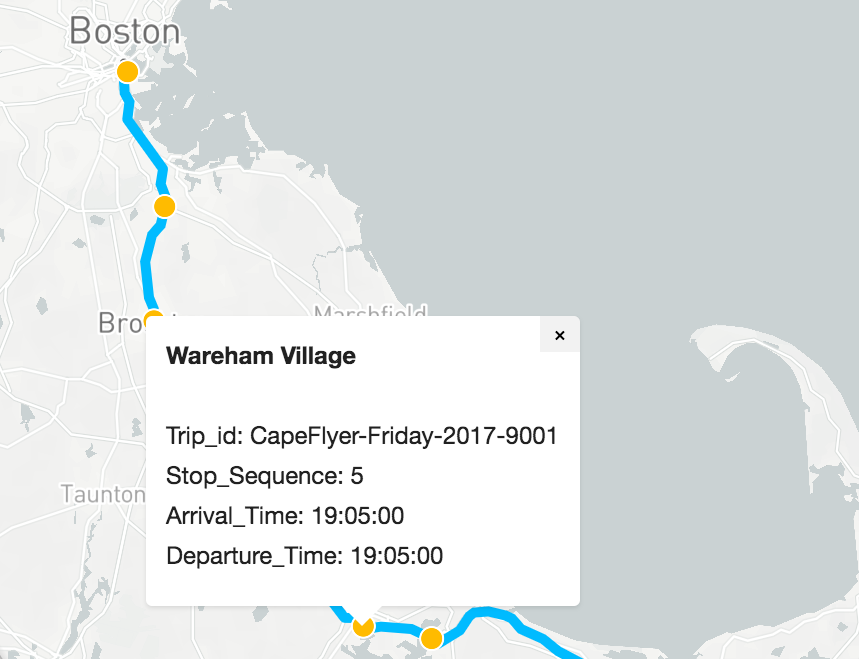
\includegraphics[width=0.5\textwidth]{prozess/add_stations}
        \caption{Hinzufügen von Stationen entlang der Polyline}
        \label{fig:prozess/add_stations}
      \end{center}
    \end{figure}

    An dieser Stelle sind bereits alle Informationen vorhanden, die benötigt werden um ein Vehicle zwischen den einzelnen Stationen fahren zu lassen. Ein Ansatz dafür, ist die Verwendung der Funktion \texttt{turf.along()}. Diese Funktion nimmt eine Polyline und gibt einen Punkt in einer bestimmten Entfernung entlang dieser Polyline zurück. Die Polyline ist bekannt, es fehlt die Distanz zwischen den einzelnen Stationen. Diese wird wie in Sektion \textit{\ref{ssub:station_matching} \nameref{ssub:station_matching}} im Backend berechnet. Des weiteren brauchen wir die Geschwindigkeit des Vehicles. Sind all diese Parameter vorhanden, lässt sich die Distanz des Vehicles (zwischen den einzelnen Stationen) zu jedem Zeitpunkt $t_i$ interpolieren.

    \begin{figure}[htbp]
      \begin{center}
        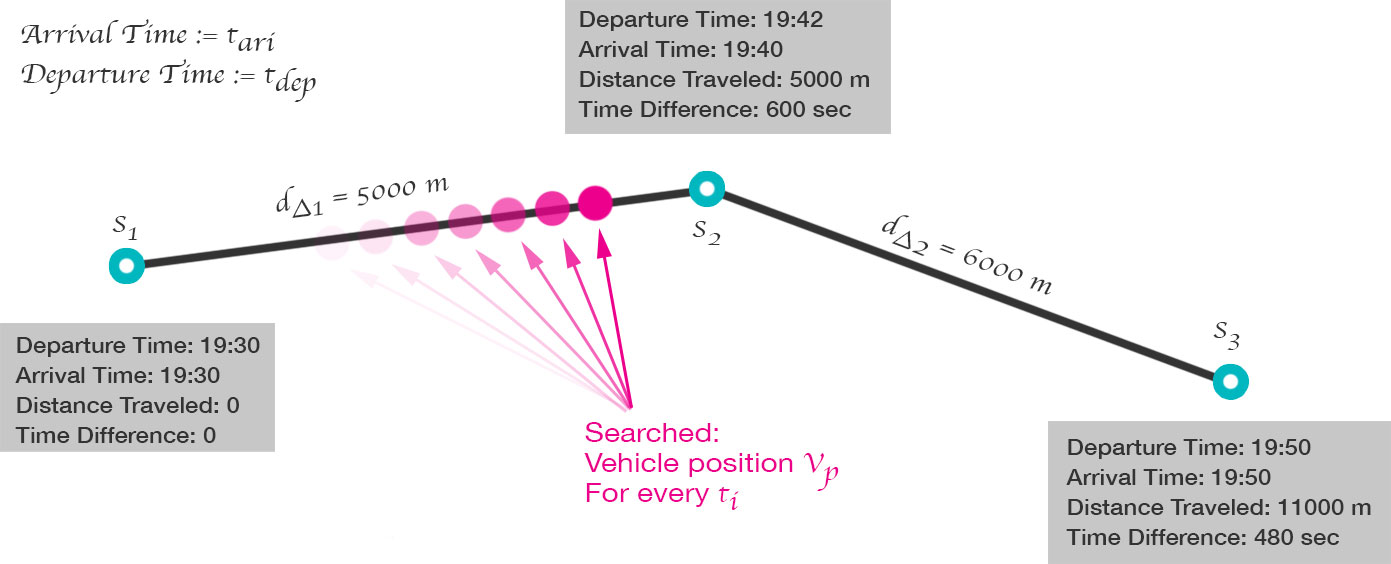
\includegraphics[width=0.9\textwidth]{interpolating_vehicle}
        \caption{Interpolation der Vehicle Position: $V_p$}
        \label{fig:interpolating_vehicle}
      \end{center}
    \end{figure}

    Die durchschnittliche Geschwindigkeit, die das Vehicle zwischen zwei Stationen hat, lässt sich über $v = \frac{d_\triangle}{TimeDifference}$ berechnen. Damit ist die Geschwindigkeit vorhanden und die interpolierte Distanz des Vehicles zu jedem Zeitpunkt $t_i$ lässt sich über die Formel der gleichförmigen Bewegung: $s_{neu} = v * t + s_0$ berechnen. Das resultierende $s_{neu}$ der Formel, kann dann an \texttt{turf.along(polyline, $s_{neu}$)} übergeben werden und gibt uns eine neue Position des Vehicles auf der Polyline zurück. Wird nun die Karte mit der neuen Position aktualisiert, fährt das Vehicle von Station zu Station. Natürlich müssen hier verschiedene Randbedingungen beachtet werden, beispielsweise was passiert, wenn das Vehicle am Ende angelangt ist oder wie werden Aufenthalte an einer Station beachtet.

    \subsection{Backend}
\label{sub:backend}
  In diesem Abschnitt soll beschrieben werden, welche Probleme beim Arbeiten mit dem GTFS Datenformat und einer PostgreSQL Datenbank bestehen und wie diese gelöst sind. Dabei steht vor allem die Behebung von Engpässen bei der Query\footnotemark Performance, als auch die Verringerung der zu verarbeitenden Datenmenge. Sektion \ref{ssub:freiräume_in_der_gestaltung_von_gtfs} beschreibt die generelle Problematik, dass durch die Verwendung des GTFS Formats im Backend entsteht. Die folgenden Abschnitte fokussieren sich darauf dieses Problem zu lösen. Abschnitt "`\nameref{ssub:gtfs_optimierungen}"' zeigt verschiedene GTFS Optimierungsschritte. Darauf folgt die Verbesserung von Polylines in Abschnitt \ref{ssub:polyline_optimieren} und endet mit der Denormalisierung von Datenbanktabellen im letzten Abschnitt \ref{ssub:denormalisierung_der_datenbank}.

  \footnotetext{Ein Query ist eine Informationsanfrage an eine Datenbank} 
  
  % Gliederung eventuell nochmals beschreiben.

  \subsubsection{GTFS Optimierungen}
\label{ssub:gtfs_optimierungen}

  Der erste Schritt um die Performance zu verbessern, ist die Optimierung von GTFS Feeds. Damit lässt sich die Datenmenge bereits vor dem Importieren in die Datenbank, erheblich verringern. Ein Tool um ein GTFS Feed umfassend zu optimieren ist \texttt{gtfstidy} \url{https://github.com/patrickbr/gtfstidy}. Es bietet dabei allerdings nicht nur die Möglichkeit für die Vereinfachung von Polylines sondern kommt mit einer ganzen Reihe an Optimierungsmöglichkeiten. 

  Der Kommandozeilenbefehl \colorbox{materialGrey}{\texttt{\color{white}{\$ gtfstidy -sSiRDeO input.zip output}}} optimiert das Stuttgart-VVS Feed wie folgt:
  
  \begin{itemize}[label={}]
    \item \textbf{-s} Reduziert die Punktanzahl einer Polyline
      
    \item \textbf{-S} Entfernt redundante Polylines.

    \item \textbf{-i} Umwandlung von Zeichen ID's (String) in Zahlen ID's (Integer).\footnote{Aus der String ID \texttt{'1.T0.10-1-j17-1.16.H'} wird \texttt{78}}

    \item \textbf{-O} Entfernt Feed Einträge die nicht referenziert werden.

    \item \textbf{-R} Entfernt doppelt vorhandene Routen.

    \item \textbf{-e} Setzt fehlerhafte oder optionale Felder auf einen Standard Wert.

    \item \textbf{-D} Entfernt fehlerhafte Einträge aus dem Feed.
  \end{itemize}

  Durch Verwendung von gtfstidy konnte das Feed optimiert werden und die Datengröße der einzelnen Dateien um folgendes Maß verringert werden.

  \begin{longtable}{|>{\raggedright \arraybackslash}p{5.0cm}|>{\raggedright \arraybackslash}p{5.0cm}|>{\raggedright \arraybackslash}p{5.0cm}|}
    \hline
    Dateiname & Größe davor& Größe danach\\
    \hline
    trips.txt & 6 MB & 2.8 MB\\
    stop\_times.txt & 103 MB & 53 MB\\
    stops.txt & 651 KB & 355 KB\\
    shapes.txt & 77.3 MB & 22.4 MB\\
    routes.txt & 54 KB & 38 KB\\
    calendar\_dates.txt & 557 KB & 463 KB\\
    \hline
    \caption{Tabellengröße bevor und nach anwenden von gtfstidy}
    \label{tbl:gtfs_tidy_results}
  \end{longtable}

  Insgesamt konnte so die Größe des Feeds von 79 MB auf 118 MB um knapp 50\% verringert werden. Vor allem die Umwandlung von langen String ID's in kürzere Integer ID's trägt maßgeblich zur Verringerung der Dateigröße bei.

% subsubsection gtfs_optimierungen (end)
  \subsubsection{Polyline optimieren}
\label{ssub:polyline_optimieren}

  Die Optimierung der Polyline ist ein sehr wichtiger Aspekt in meiner Arbeit und soll in diesem Abschnitt vertieft werden.

  \subsubsection*{Ramer–Douglas–Peucker}
  \label{ssub:ramer_douglas_peucker}
    Das Problem: Die im Stuttgart-VVS Feed zur Verfügung gestellten Polylines sind Überdefiniert und können aus tausenden Punkten bestehen. Für eine Visualisierung ist eine solche Genauigkeit nicht notwendig und aufgrund der großen Datenmenge problematisch. Im vorigen Abschnitt \ref{ssub:gtfs_optimierungen} wurde die Option \colorbox{materialGrey}{\texttt{\color{white}{-s}}} vorgestellt. Dieser Befehl verwendet den "`Ramer–Douglas–Peucker"' (RDP) Algorithmus um die Anzahl der Punkte einer Polyline zu reduzieren. Der Vorteil besteht darin, dass dabei nicht der Linienverlauf verändert wird. Abbildung~\ref{fig:simplify} zeigt ein Beispiel einer solchen Vereinfachung mittels einer JavaScript Bibliothek\footnote{Simplify.js \url{http://mourner.github.io/simplify-js/}}.

    \begin{figure}[htbp]
      \centering
      \subfloat[Polyline vor RDP]{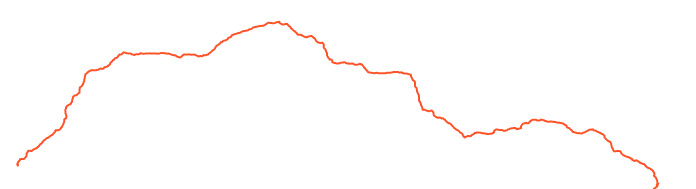
\includegraphics[width=0.48\textwidth]{simplify_before.jpg}\label{fig:simplify_before}}
      \hfill
      \subfloat[Polyline nach RDP]{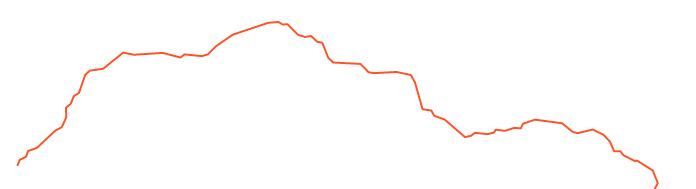
\includegraphics[width=0.48\textwidth]{simplify_after.jpg}\label{fig:simplify_after}}
      \caption{Vereinfachung einer Polyline mittels Simplify.js}
      \label{fig:simplify}
    \end{figure}

    Ausgangspunkt ist eine Polyline mit $\approx1000$ Punkten (\ref{fig:simplify}a). Nach der Vereinfachung (\ref{fig:simplify}b) ist die Anzahl auf 100 Punkte reduziert, ohne dabei visuell merklich einzubüßen. Dies ist eine erhebliche Reduzierung der Punkte um 90\%. Wie wirkt sich dieser Algorithmus positiv auf das Projekt aus? Die Vorteile sind weitreichend. Sehen wir uns die Shape Tabelle in Abbildung \ref{fig:shape_simplify} an. \ref{fig:shape_simplify}a zeigt 394 Reihen vor der Optimierung und nur noch 140 (\ref{fig:shape_simplify}b) nach Anwendung von gtfstidy.

    \begin{figure}[htbp]
      \centering
      \subfloat[Shapte Tabelle vor RDP]{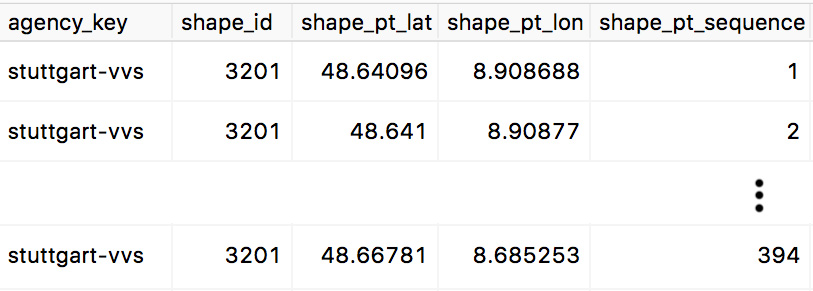
\includegraphics[width=0.48\textwidth]{shape_simplify_before.jpg}\label{fig:shape_simplify_before}}
      \hfill
      \subfloat[Shapte Tabelle nach RDP]{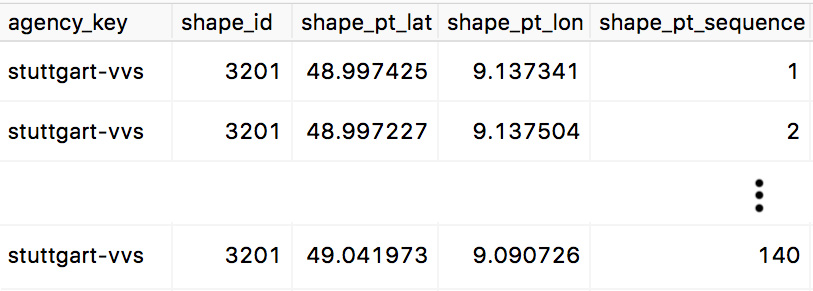
\includegraphics[width=0.48\textwidth]{shape_simplify_after.jpg}\label{fig:shape_simplify_after}}
      \caption{Reduzieren der Polyline via gtfstidy}
      \label{fig:shape_simplify}
    \end{figure}

    In seinem Originalzustand hat das verwendete VVS Feed 1,085,859 Mio Zeilen. Nach der Anwendung sind diese auf 617,653 Tsd. verringert. Testet man folgende PostgreSQL Abfrage
    \colorbox{materialGrey}{\texttt{\color{white}{{\color{materialBlue}SELECT} * {\color{materialBlue}FROM} gtfs\_shapes {\color{materialBlue}WHERE} shape\_id = {\color{materialRed}3201}}}}
    die alle Punkte einer Polyline ausgeben soll, so ergibt sich für ein optimiertes Feed eine Query Zeit von $\approx145 ms$ und für das nicht optimierte Feed $\approx250 ms$. Schon durch diese einfache Methode sind bereits erste Performance Steigerungen wahrnehmbar.

  % subsubsection ramer_douglas_peucker (end)

  \subsubsection*{Aggregieren der Shape Tabelle}
  \label{ssub:aggregieren_der_shape_tabelle}
    In GTFS wird für jeden Punkt einer Polyline eine Reihe in der Datenbank belegt. Diese Abfolge ist durch eine sogenannte \texttt{Shape Point Sequence} festgelegt, was nichts anderes ist als eine Zahl von $1$ bis $n$. Dies ist auch bereits in obiger Tabelle \ref{fig:shape_simplify} zu sehen gewesen. Sehr viel effektiver wäre es allerdings, diese Punkte nicht Reihenweise zu speichern, sondern alle zusammen gehörenden Punkte in einem einzigen Feld zu speichern. Dies ist in PostgreSQL durch eine Aggregierung möglich. Daraus ergibt sich folgende Shape Tabelle:

    \begin{figure}[htbp]
      \begin{center}
        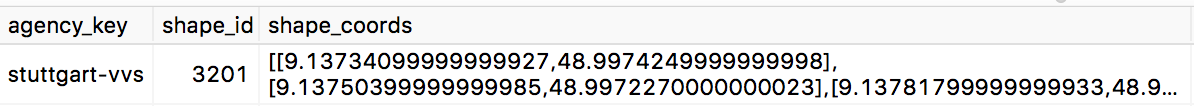
\includegraphics[width=\textwidth]{aggregated.png}
        \caption{Aggregierte Koordinaten der Shape Tabelle}
        \label{fig:aggregated}
      \end{center}
    \end{figure}

    Wie zu sehen ist benötigt nun eine Polyline in der Shape Tabelle nicht mehr 140 Reihen, sondern nur noch eine einzige. Für diese Arbeit ist dies auf alle Polylines angewendet worden und in einer neuen Tabelle namens \texttt{denormalized\_shapes} abgespeichert. Dadurch ist die Berechnung der Aggregierung nur einmal nötig. Der SQL-Befehl dafür ist dem Anhang unter \ref{lst:sql_aggregate_shape}. zu entnehmen.
    Wenden wir die selbe SQL Abfrage, die bereits oben Verwendung fand, auf die neue \texttt{denormalized\_shapes} Tabelle an. Die Query Zeit ist auf $\approx1ms$ gesunken! Anstatt hunderte Reihen muss nur eine einzige Reihe ausgelesen werden, was sehr sehr schnell ist. Durch das Denormalisieren\footnotemark der Shape Tabelle ist auch die Anzahl der Reihen auf ein Minimum gesunken. Von den früheren 617,653 Tsd. Reihen, sind jetzt durch die Aggregation nur noch 4,524 Tsd. übrig.

    \footnotetext{Denormalisieren beschreibt den Prozess der Relationsauflösung von Datenbanktabellen.}
  
  % subsubsection aggregieren_der_shape_tabelle (end)

  \subsubsection*{Polyline Encoding}
  \label{ssub:polyline_encoding}
    Die letzte Maßnahme zur Optimierung der Polyline stellt das sogenannte Polyline Encoding dar. Wie dieses Verfahren genau funktioniert, geht an dieser Stelle zu weit. Hier soll nur erklärt werden, was das Polyline Encoding für diese Arbeit bedeutet und warum es verwendet wird.\\

    Das Polyline Encoding kann in JavaScript beispielsweise durch das Google-Polyline\footnote{\url{https://www.npmjs.com/package/google-polyline}} Paket eingesetzt werden. Das Encoding wandelt eine Polyline, bestehend aus Punkten, in einen String um. Zum Beispiel die Punkte: (38.5, -120.2), (40.7, -120.95), (43.252, -126.453) werden als
    \colorbox{materialGrey}{\texttt{\color{white}{\_p\textasciitilde iF\textasciitilde ps|U\_ulLnnqC\_mqNvxq`@}}}
    codiert. Dies geschieht in meiner Anwendung immer genau dann, bevor Daten von Server in Richtung Client geschickt werden: Encode $\rightarrow$ Send $\rightarrow$ Decode. Da eine codierte Polyline weniger Zeichen benötigt, kann damit Datenvolumen bei der Kommunikation zwischen Server und Client gespart werden.

  % subsubsection polyline_encoding (end)


% subsubsection polyline_optimieren (end)
  \subsubsection{Denormalisierung der Datenbank}
\label{ssub:denormalisierung_der_datenbank}
  Die Denormalisierung ist eine Strategie, die auf eine zuvor normalisierte Datenbank angewendet wird, um die Leistung zu erhöhen. Die Denormalisierung ist der Prozess, bei dem versucht wird, die Leseperformance einer Datenbank zu verbessern, auf Kosten der Schreibleistung, durch Hinzufügen redundanter Kopien von Daten oder durch deren Gruppierung.\parencite{sanders}
  Der große Nachteil von Denormalisierung, nämlich die Redundanz von Daten, spielt für dieses Projekt keine Rolle, da die Daten ausschließlich ausgelesen und nicht geschrieben werden. Was bleibt sind die Vorteile.\\

  Für dieses Projekt bedeutet diese Methode, eine neue Tabelle zu generieren, die den Zugriff auf die benötigten Daten einfach macht. Im Grunde handelt es sich um eine Vorberechnung. Anstatt die Tabellen bei jeder Anfrage an den Server aufwendig über viele \texttt{SQL-JOINS} zu verknüpfen, wird diese Verknüpfungen einmalig vorberechnet und in eine Tabelle gespeichert. Eine Denormalisierung  einer Tabelle ist bereits im vorherigen Abschnitt "`\nameref{ssub:aggregieren_der_shape_tabelle}"' gezeigt und führte dazu, dass die Polyline über die Abfrage einer einzigen Tabellenreihe erhalten werden kann was die Performance signifikant erhöhte. Zur besseren Verständnis soll folgende Grafik helfen:

  \begin{figure}[htbp]
    \begin{center}
      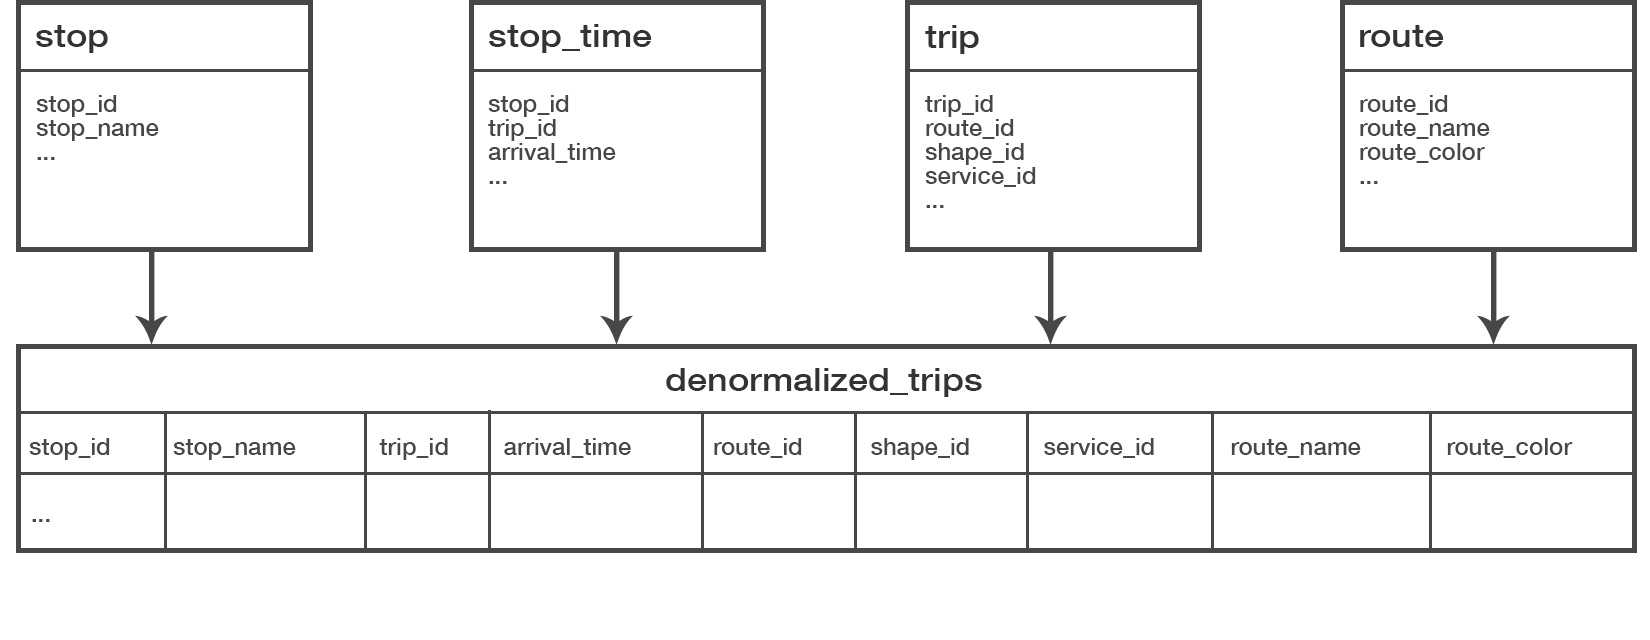
\includegraphics[width=\textwidth]{denormalizing.jpg}
      \caption{Beispiel einer Denormalisierung von Tabellen}
      \label{fig:denormalizing}
    \end{center}
  \end{figure}

  Wie in Abbildung \ref{fig:denormalizing} zu sehen ist, wird aus einer vertikalen Anordnung der einzelnen Datenfelder, eine horizontale Anordnung in einer einzigen \texttt{denormalized\_trips} Tabelle. Eine Reihe in dieser neuen Tabelle steht für genau einen Eintrag eines Trips. Anstatt also bei jeder Anfrage an den Server die verschiedenen Daten mittels \texttt{JOIN} verknüpfen zu müssen, können diese jetzt per Zugriff auf eine einzige Reihe in nur einer Tabelle erfragt werden.\\

  Dieses Prinzip, der Gruppierung von Daten in einer neuen Tabelle soll nun auch auf die anderen benötigten Tabellen angewendet werden. Die Denormalisierung erfolgt in 3 Schritten:

  \begin{enumerate}
    \item Erstellen der neuen Tabelle \texttt{denormalized\_trips}
    \item Importieren der verschiedenen Daten in diese neue Tabelle
    \item Mögliche Abfragen sind nun über diese neue Tabelle möglich.
  \end{enumerate}

  Das SQL-Statement ist abermals aufgrund seiner Länge Anhang \ref{lst:denormalized_shapes} zu entnehmen. Dies resultiert in einer Tabelle die wie folgt aussieht:

  \begin{figure}[htbp]
    \begin{center}
      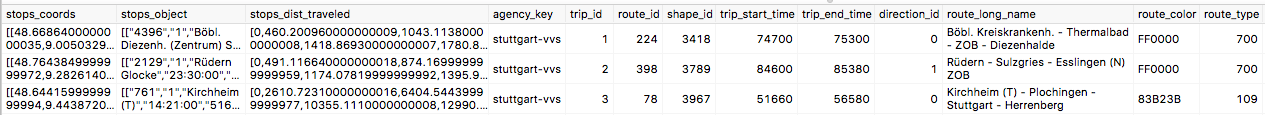
\includegraphics[width=\textwidth]{denormalized_tables.png}
      \caption{Auszug aus der \texttt{denormalized\_trips} Tabelle}
      \label{fig:denormalized_table}
    \end{center}
  \end{figure}  

  \subsubsection*{Ergebnisse der Denormalisierung}
  \label{ssub:ergebnisse_der_denormalisierung}
    Für die Visualisierung ist eine Abfrage der aktiven Trips am wichtigsten.
    Folgende Tabellen werden für die Abfrage benötigt.

    \begin{figure}[htbp]
      \begin{center}
        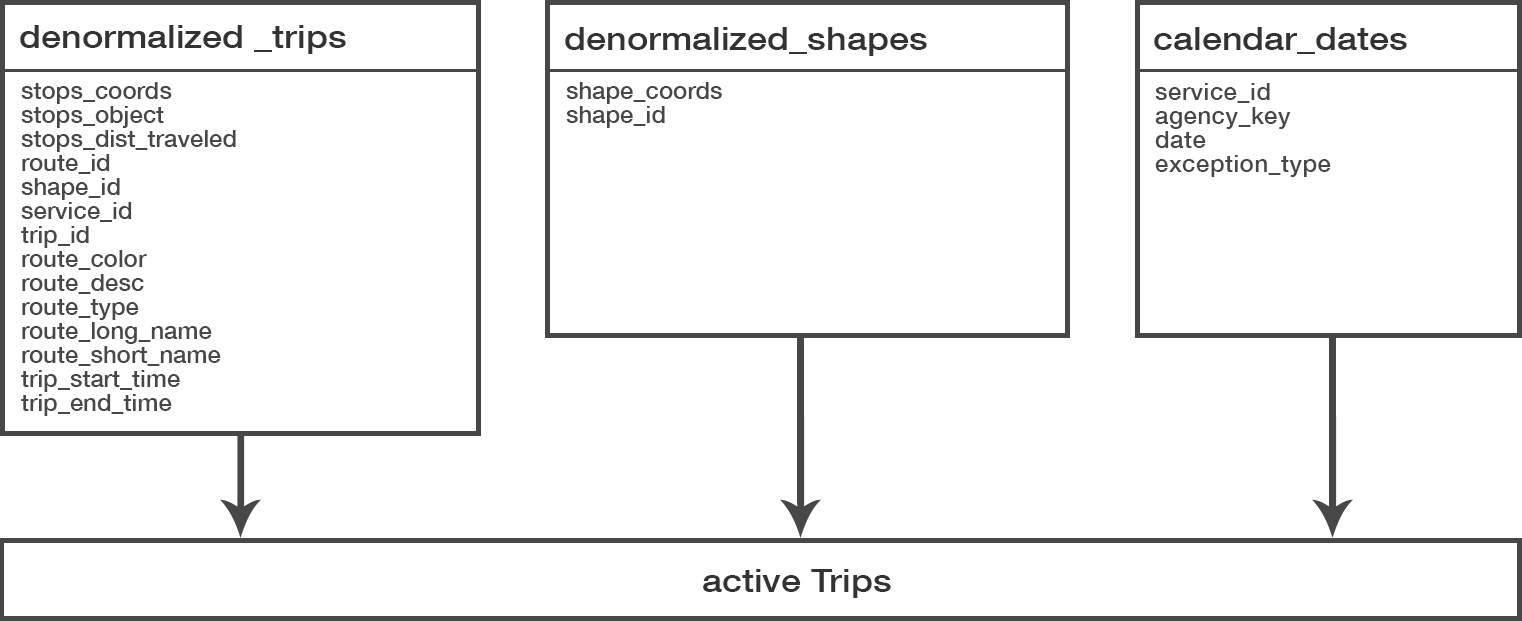
\includegraphics[width=\textwidth]{denormalizing_results.jpg}
        \caption{Benötigte Tabellen zur Abfrage von Trips}
        \label{fig:denormalizing_results}
      \end{center}
    \end{figure}

    Wie zu sehen ist, wird auf die Denormalisierte \texttt{Shape} und \texttt{Trips} Tabelle zugegriffen.

    Nachfolgend die Ergebnisse für die Abfrage von Trips in einem wachsenden Zeitrahmen. Die verwendete SQL-Abfrage befindet sich im \nameref{sec:anhang} unter Listing \ref{lst:query_trips}.

    \begin{longtable}{|>{\raggedright \arraybackslash}p{5.0cm}|>{\raggedright \arraybackslash}p{5.0cm}|>{\raggedright \arraybackslash}p{4.0cm}|}
    \caption{Evaluierung der Denormalisierung}\label{tbl:evaluierung_der_denormalisierung}\\
      \hline
        Zeitraum & Trip Anzahl & Query Zeit\\
      \hline
        9:00 bis 9:15 & 88 & 98 ms\\
        9:00 bis 10:00 & 1125 & 154 ms\\
        9:00 bis 12:00 & 3360 & 285 ms\\
        9:00 bis 15:00 & 7070 & 497 ms\\
        9:00 bis 21:00 & 14718 & 900 ms\\
      \hline
    \end{longtable}

    Die Ergebnisse Zeigen, dass die Abfragezeit der Datenbank für die aktiven Trips erheblich gesunken ist. Anfangs ist solch eine Anfrage aufgrund der endlosen Laufzeit erst gar nicht möglich gewesen.

    \begin{figure}[htbp]
      \begin{center}
        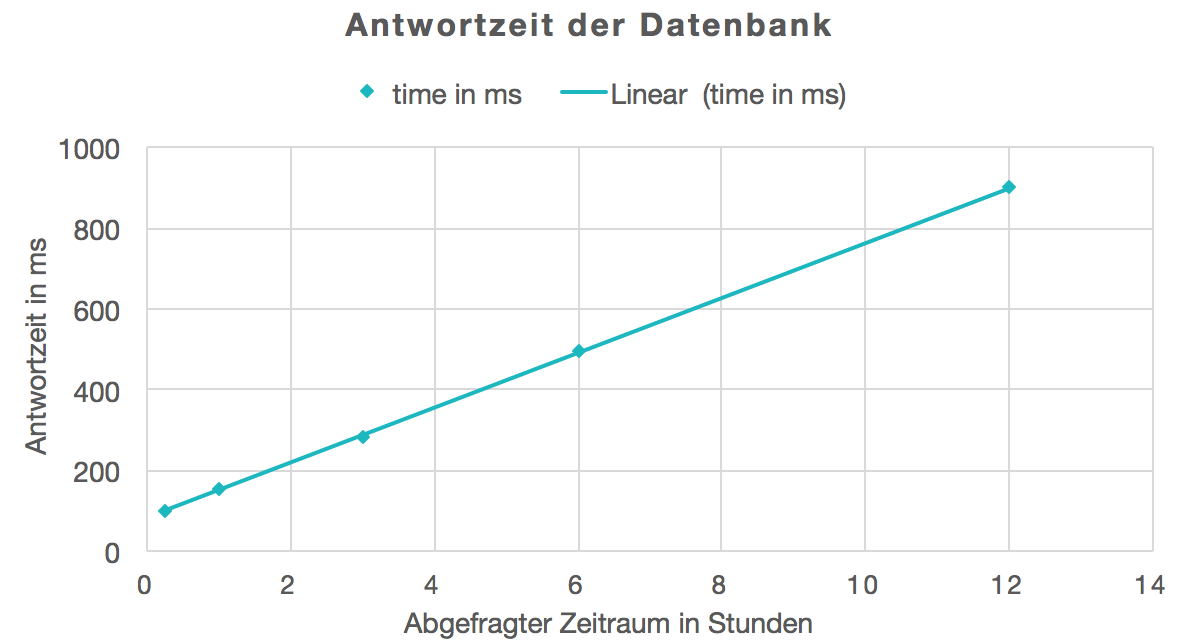
\includegraphics[width=0.65\textwidth]{query_time_chart}
        \caption{Plot der Abfragezeiten}
        \label{fig:query_time_chart}
      \end{center}
    \end{figure}
    
    Abbildung \ref{fig:query_time_chart} zeigt einen Plot der Query Zeit aus Tabelle \ref{tbl:evaluierung_der_denormalisierung} als nahezu linearen Graphen. Daraus folgt, dass die Antwortzeit der Datenbank linear mit dem abgefragten Zeitraum wächst. In der Visualisierung sind vor allem Trip Abfragen zwischen einer Minute und einer Stunde in Verwendung. Die Abfragezeit bewegt sich damit zwischen $\approx 80 -  160\; ms$.
    
  % subsubsection ssub:ergebnisse_der_denormalisierung (end)

% subsubsection denormalisierung_der_datenbank (end)
  \subsubsection{API Endpunkte}
\label{ssub:api_endpunkte}
  Um einen Datenaustausch zwischen Server und Client zu ermöglichen, sind folgende API\footnotemark Endpunkte vorhanden. 

  \footnotetext{Application Programming Interface}

  \begin{itemize}[label={}]
    \item \textbf{/daily} Stellt die Daten für das Zeitstrahldiagramm bereit. Wird beim Start der Anwendung einmalig Angefragt. Die Antwort enthält XY-Wertpaare. X stellt dabei die Zeit in Sekunden und Y die zu diesem Zeitwert aktiv werdenden Trips dar.

\begin{lstlisting}[captionpos=t, caption=Antwort des Servers zur Anfrage \texttt{/daily}, label=lst:daily_response]
[
  {"x":86340,"y":"6"},
  {"x":86400,"y":"10"}, 
  ...
]
\end{lstlisting}

    \item \textbf{/trips/:from,:to} Ermöglicht das Abfragen von Trips, die in einer Zeitspanne \texttt{from - to} aktiv sind. Beim initialen Aufruf der Webanwendung wird dieser Endpunkt als erstes angefragt um die aktiven Trips innerhalb einer Stunde zu bekommen. Der gewählte Zeitraum ist in Sekunden anzugeben. Die Definition ist wie folgt: $t_{from} = now$ und $t_{to} = now + 600 sec$. Die Sekunden lassen sich nach der Formel aus Kapitel \ref{ssub:time} berechnen.
     durch das Addieren der Stunden, Minuten und Sekunden errechnen. Bsp: 17:04:59 Uhr

    $\Rightarrow t_{from} = 61499 \Rightarrow t_{to} = 61499 + 600\;sec$ $\Rightarrow$ \texttt{/trips/61499,62099}

    Die Antwort des Servers auf einen Endpunkt vom Typ \texttt{/trips/} ist ein Objekt mit der Trip\_Id, dessen Inhalt der \texttt{GeoJSON} spezifikation nach RFC 7946 folgt:

\begin{lstlisting}[captionpos=t, caption=Trip Objekt, label=lst:trip_object]
{
  2498: {  
    "type": "FeatureCollection",
    "features": [
      {
        "type": "Feature",
        "properties": {
          "name": "shape",
          ...
        },
        "geometry": {
          "type": "LineString",
          "coordinates": [[9.4437,48.64482], ...]
        }
      },
      {
        "type": "Feature",
        "properties": {
          "name": "station"
        },
        "geometry": {
          "type": "Point",
          "coordinates": [9.443688, 48.6448]
        }
      },
      ...
    ]
  }
}
\end{lstlisting}
  
    Da die Antwort in Listing \ref{lst:trip_object} mittels "`..."' gekürzt ist, sind detailiertere Antworten im \nameref{sec:anhang} unter Listing \ref{lst:geojson_featurecollection}, \ref{lst:shape_feature} und \ref{lst:station_feature} zu finden.
  

    \item \textbf{/trips/:id} Antwortet mit den zur ID gehörenden Trip Informationen. Dieser Endpunkt ermöglicht es, Informationen für nur einen einzigen Trip zu bekommen. Dies ist vor allem dann hilfreich, wenn der Nutzer ein Vehilce anklickt und Informationen über diesen Trip angezeigt bekommen möchte. Beispiel: \texttt{/trips/51295}

    \item \textbf{/trips/new/:from,:to,:tripIds} Stellt die Abfrage für neue Trips zur Verfügung und exkludiert dabei diejenigen Trips, die in \texttt{:tripIds} genannt sind. Damit wird verhindert, dass bereits auf der Karte vorhandene Trips nicht doppelt auftauchen können. Dieser Query wird in einem 30 Sekunden Intervall vom Client an den Server gesendet um die neusten Trips zu erhalten. Damit wird die Karte aktuell gehalten. Beispiel: Es ist 10:00 Uhr, hole die in der nächsten Minute aktiv werdenden Trips (Zeitraum 10:00 bis 10:01 Uhr) und schließe die Trips mit der ID \texttt{51295,9212,52} vom Ergebnis aus \texttt{/trips/new/36000,36060,51295,9212,52}.

    \item \textbf{/trips/new/:from,:to} Stellt die gleiche Funktionalität wie der vorherige Endpunkt zur Verfügung, mit der Ausnahme, dass keine Trip-ID's übermittelt werden müssen. Dieser Endpunkt ist beispielsweise dafür da, falls die Karte leer ist und noch keine aktiven Trips enthält.

  \end{itemize}

% subsubsection api_endpunkte (end)
  \subsubsection{Server}
\label{ssub:server}
  Der Nodejs Server stellt die zuvor definierten Endpunkte mittels \texttt{Express.js} als ansprechbare Routen dem Client zur Verfügung. Express ist ein minimalistisches Node.js Framework für moderne Web Applikationen. Es vereinfacht die Erstellung von API Endpunkten durch das Bereitstellen hilfreicher Methoden zur Erstellung von Routen\footnotemark.

  \footnotetext{Routing refers to determining how an application responds to a client request to a particular endpoint, which is a URI (or path) and a specific HTTP request method (GET, POST, and so on). \url{https://expressjs.com/en/starter/basic-routing.html}}

  \begin{figure}[htbp]
    \begin{center}
      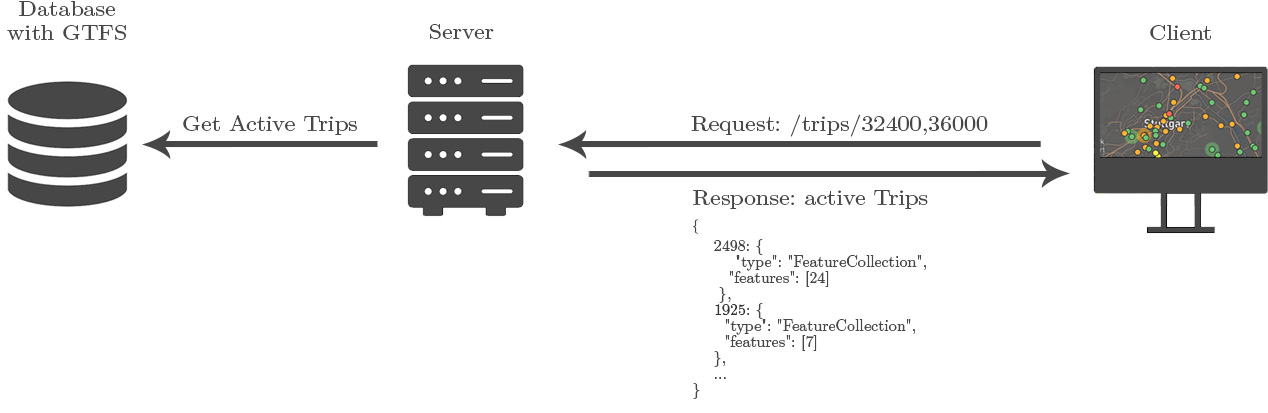
\includegraphics[width=\textwidth]{server_client.jpg}
      \caption{Server / Client Relation}
      \label{fig:server_client}
    \end{center}
  \end{figure}

  Trifft eine valide Anfrage auf den \texttt{/trips/:from,:to} Endpunkt, so wird ein Ablauf nach Abbildung \ref{fig:server_client} angestoßen.
  Die eintreffenden Anfragen werden vom Server entgegengenommen, validiert, verarbeitet und anschließend die entsprechende Antwort zurück gesendet. Die Validierung prüft die vom Client übergebenen Parameter auf ihre Plausibilität. Schlägt diese Prüfung fehl wird ein Fehler vom Server zurückgegeben und der Server wartet auf eine neue Anfrage. Die wichtigste Routine des Servers stellt die Abfrage von Trips aus der Datenbank dar. Die Datenbank sucht diejenigen Trips heraus, welche in dem benötigten Zeitraum \texttt{from, to} aktiv sind. Dabei wird das Datum und der Wochentag zum Zeitpunkt der Anfrage verwendet. Damit der Client bei der Animation möglichst wenig Rechenarbeit hat, werden alle Daten, bei denen dies möglichst ist, vorberechnet. Folgender Ablauf findet statt:

  \begin{itemize}
    \item \textbf{Daten Mapping:} Die Trips aus der Datenbank werden in das \texttt{GeoJSON}-Format umgewandelt, damit diese im weiteren Programmverlauf einfacher zu verarbeiten sind. Dabei werden die im Kapitel "`\ref{sub:begriffe} \nameref{sub:begriffe}"' festgelegten Definitionen beachtet.

    \item \textbf{Zurückgelegte Distanz:} Damit eine Animation der Vehicle stattfinden kann ist die Berechnung der Distanzen zwischen den einzelnen Stationen nötig. Falls das Feld \texttt{stops\_dist\_traveled}\footnotemark in der Datenbank vorhanden ist, kann die zurückgelegte Distanz sehr einfach daraus berechnet werden. Ist dies nicht der Fall so wird ein Station Matching durchgeführt, um die Distanzen berechnen zu können.
    \footnotetext{Die zurückgelegte Distanz bis zu einer Station $S$}

    \item \textbf{Station Matching:} Unter Station Matching versteht sich die Positionierung der Stationen auf und entlang der Polyline. Dies wird im nächsten Abschnitt ausführlicher betrachtet.

    \item \textbf{Feststellen der Richtung:} Für eine Polyline ist es unerheblich ob die Koordinaten in der Reihenfolge $\{ p_1, p_2, \dotsc, p_n \}$ oder $\{ p_n, \dotsc, p_2, p_1 \}$ angeordnet sind. Damit das Vehicle aber in die richtige Richtung von $A$ nach $B$ fährt, ist es wichtig dass die Koordinaten der Polyline in aufsteigender Reihenfolge festgelegt werden. Falls dies nicht er Fall ist, werden die Koordinaten in ihrer Reihenfolge umgekehrt.

    \item \textbf{Codieren der Polyline:} Zuletzt werden die Koordinaten in einen Polyline String Codiert und abschließend versendet.
  \end{itemize}

% subsubsection server (end)
  \subsubsection*{Station Matching}
\label{ssub:station_matching}

  Das Station Matching war eines der fundamentalen Herausforderungen bei der Programmierung des Servers. Es ist dafür da, um die Distanz zwischen den einzelnen Stationen zu ermitteln. Zwar hat das Stuttgart-VVS Feed ein \texttt{stop\_distance\_traveled} Feld, welches die benötigten Distanz Informationen direkt aus der Datenbank liefert, aber für andere GTFS-Feeds die getestet wurden, ist dieses Feld oftmals nicht vorhanden. Die Applikation verwendet also das \texttt{stop\_distance\_traveled} Feld, falls es vorhanden ist und als Fallback-Lösung erfolgt die Berechnung via Station Matching Algorithmus.\\

  Das Station Matching soll folgendes Problem lösen:

  \begin{figure}[htbp]
    \begin{center}
      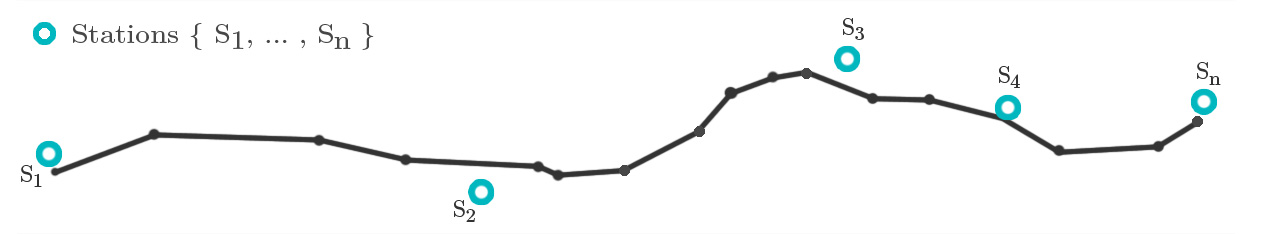
\includegraphics[width=\textwidth]{station_problem.jpg}
      \caption{Stationen liegen nicht direkt auf der Polyline}
      \label{fig:station_problem}
    \end{center}
  \end{figure}
  
  Wie in Grafik \ref{fig:station_problem} zu sehen ist liegen die Stationen nicht exakt auf der Polyline, sondern sind ein wenig abseits platziert. So entspricht die Position der Station einer Haltestelle oder Bahnhof. Meistens befinden sich diese ein wenig versetzt zum eigentlichen Verlauf der Strecke. Die Visualisierung interpoliert die Bewegung eines Vehicles zwischen den einzelnen Stationen. Damit das möglich ist, wird die zurückzulegende Distanz zwischen den einzelnen Stationen benötigt. Um sie zu berechnen ist es nötig die Stationen auf die Polyline zu legen (das Matching).

  \begin{figure}[htbp]
    \begin{center}
      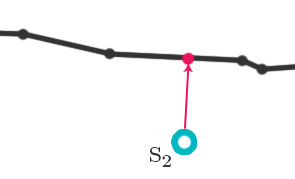
\includegraphics[width=0.25\textwidth]{find_nearest_point}
      \caption{Finde den am nächstgelegenen Punkt der Station auf der Polyline}
      \label{fig:find_nearest_point}
    \end{center}
  \end{figure}

  Nachdem ein Punkt auf der Polyline gefunden ist, kann die Distanz berechnet werden. Die Distanzen zweier Stationen $\{s_i,s_{i+1} \;|\; i \in \mathbb{N} \}$ sei $d_\triangle$. Diese kann jetzt wie folgt berechnet werden: $ d_\triangle = d_{i+1} - d_i$. 

  \begin{figure}[htbp]
    \begin{center}
      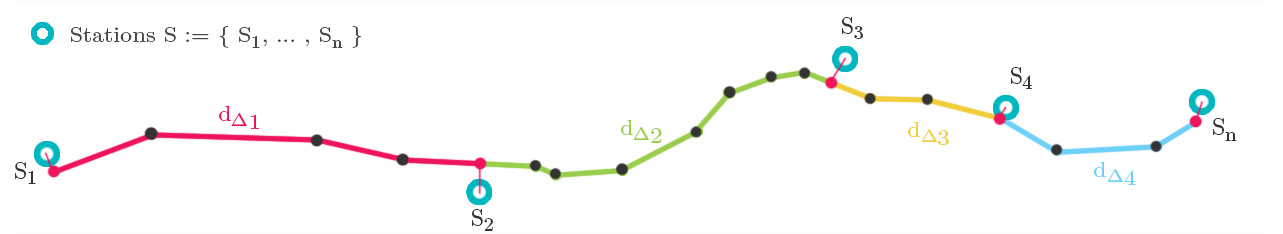
\includegraphics[width=\textwidth]{get_distances}
      \caption{Berechnen der Distanz}
      \label{fig:get_distances}
    \end{center}
  \end{figure}
  
  In Listing \ref{lst:match_station} des Anhangs wird ein Algorithmus vorgestellt, der das Problem des Station Matchings und der Distanzberechnung löst. Abbildung \ref{fig:station_matching_comparision} stellt eine frühere Implementierung mit der nun aktuellen Version des Algorithmus gegenüber. Dafür wird Zeit, die der jeweilige Algorithmus zum Matching über $n$-Trips benötigt verglichen. Um eine durchschnittliche Laufzeit zu erhalten wurde jeder Algorithmus 10 mal mit der gleichen Anzahl an Trips ausgeführt.

  \begin{figure}[htbp]
    \begin{center}
      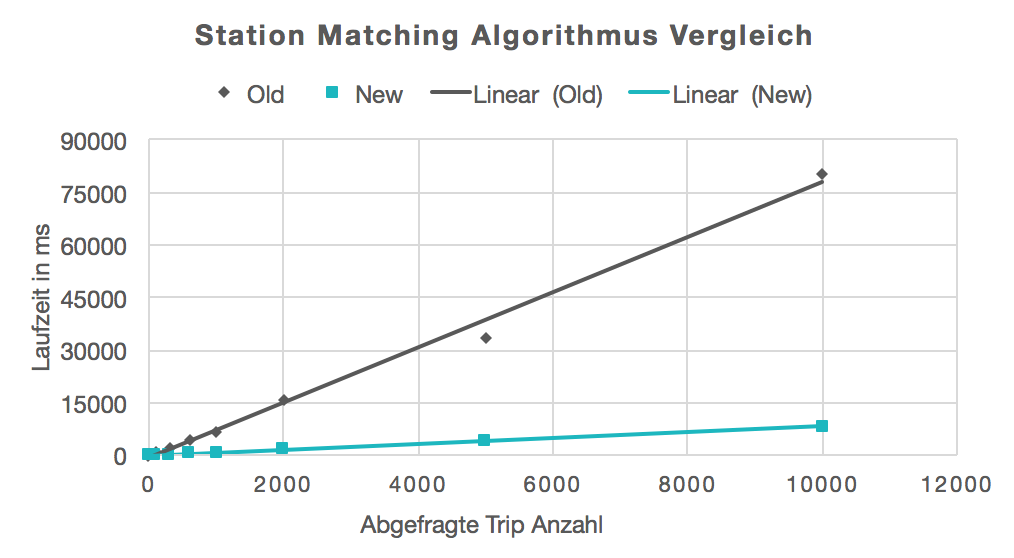
\includegraphics[width=0.7\textwidth]{station_matching_comparision}
      \caption{Vergleich der zwei Station Matching Algorithmen}
      \label{fig:station_matching_comparision}
    \end{center}
  \end{figure}

  Der alte Algorithmus war sehr simpel und beruhte darauf die Funktion \texttt{pointOnLine} der \texttt{Turf.js} Bibliothek zu verwenden. Diese Funktion hatte den entscheidenden Nachteil, dass sie in 3 \texttt{for}-Schleifen über die gesamten Punkte der Polyline iteriert. Hinzu kommt, dass das Matching nicht nur auf eine Station, sondern auf sämtliche Stationen aus allen Trips angewendet werden muss. Das führte dazu, dass insgesamt 5 \texttt{for}-Schleifen verwendet wurden. Damit lässt sich der im Vergleich höhere Anstieg der Laufzeit bei steigender Trip Anzahl erklären.

  Generell ist der neue Algorithmus sehr viel schneller. Durch die Verwendung eines \texttt{R-Trees}\footnotemark und der eigenen Implementierung verschiedener Bibliotheksfunktionen, konnte die Laufzeit drastisch reduziert werden (siehe Tabelle \ref{tbl:station_matching_comparison}). 

  \begin{longtable}{|>{\raggedright \arraybackslash}p{5.0cm}|>{\raggedright \arraybackslash}p{5.0cm}|>{\raggedright \arraybackslash}p{5.0cm}|}
  \caption{Station Matching Vergleich Old / New}\label{tbl:station_matching_comparison}\\
    \hline
    Anz. verarbeiteter Trips & Old (in ms)& New (in ms)\\
    \hline
    100    & 712   & 121  \\
    300    & 2191  & 305  \\
    600    & 4344  & 545  \\
    1.000  & 6780  & 874  \\
    2.000  & 15782 & 1700 \\
    5.000  & 33708 & 4161 \\
    10.000 & 80291 & 8279 \\
    \hline
  \end{longtable}

  Zwar wachsen beide Implementierungen lediglich Linear mit steigender Trip Anzahl, allerdings benötigt der neue Algorithmus für die Verarbeitung von $10.000$ Tausend Trips anstatt $80.29$ nur $8.28$ Sekunden.  

  Im Realbetrieb verarbeitet der Server zwischen $0 - 500$ Trips. Bei dieser Anzahl beträgt die Laufzeit des Algorithmus $\approx80ms - 400ms$. Dadurch kann argumentiert werden, dass der Algorithmus gerade noch schnell genug für eine Webanwendung arbeitet. Auch größere Anzahlen an Trips wären noch in akzeptabler Geschwindigkeit berechenbar. So können $1000$ Trips immer noch in unter einer Sekunde berechnet werden. Allerdings wäre es bei einer größeren Anzahl an Trips, der falsche Ansatz diese bei jeder Serveranfrage zu kalkulieren. Besser wäre es, einmalig das Matching für alle Trips eines GTFS Feeds durchzuführen und die Ergebnisse persistent in der Datenbank abzuspeichern. Dies könnte beispielsweise gleich beim Importieren der Daten in die Datenbank geschehen. Dadurch kann die Berechnung komplett eingespart werden. Da für das Stuttgart-VVS Feed glücklicherweise die zurückgelegte Distanz bis zu einer Station, bereits zur Verfügung steht, muss nur noch die Distanz zwischen den Stationen ($d\triangle$) berechnet werden. Dies geschieht nach dem selben Prinzip wie in der oben genannten Formel: $ d_\triangle = d_{i+1} - d_i$. Diese Berechnung ist trivial und erfolgt bei $10.000$ Trips in unter 15 Millisekunden.

  \footnotetext{Ein R-Tree (R für Rectangle) bezeichnet eine Baumförmige Datenstruktur für das Speichern und Abfragen von raumbezogenen Informationen. In Verwendung ist folgende Bibliothek: \url{https://github.com/mourner/rbush}}
  
% subsubsection station_matching (end)
  \subsubsection{Backend Performance}
\label{ssub:backend_performance}
  In diesem Abschnitt soll das gesamte Backend (Server und Datenbank) evaluiert werden. Dazu werden sowohl die Zeit zum Abfragen der Datenbank, als auch die Zeit zur Datenverarbeitung auf dem Server betrachtet werden.

  \begin{longtable}{|>{\raggedright \arraybackslash}p{4.5cm}|>{\raggedright \arraybackslash}p{1.2cm}|>{\raggedright \arraybackslash}p{1.2cm}|>{\raggedright \arraybackslash}p{1.2cm}|>{\raggedright \arraybackslash}p{1.2cm}|>{\raggedright \arraybackslash}p{1.2cm}|>{\raggedright \arraybackslash}p{1.2cm}|}
  \caption{Backend Evaluation}\label{tbl:backend_evaluation}\\
    \hline
    Anz. Trips & 20 & 100 & 500 & 1000 & 5000 & 10000\\
    \hline
    Query Zeit (ms)        & 25 & 88 & 124 & 200 & 855 & 1631 \\
    Verarbeitungszeit (ms) & 2 & 27 & 40 & 142 & 226 & 435 \\
    Summe (ms)             & 27 & 115 & 164 & 342 & 1081 & 2066 \\
    \hline
  \end{longtable}

  In Tabelle \ref{tbl:backend_evaluation} sind die Datenwerte für verschiedene Abfragen aufgelistet. Die Werte ergeben sich aus dem Mittelwert der Laufzeit in 10 Durchläufen. Wie bereits in Kapitel "`\nameref{ssub:bewältigung_der_datenmenge}"' festgestellt:

  \begin{quote}
    \textit{"`In einer Minute [werden] minimal 0 und maximal 27 Vehicle aktiv. Im Schnitt starten 9 Vehicles pro Minute ihre Fahrt."'}\ref{ssub:bewältigung_der_datenmenge}
  \end{quote}

  Aus dieser Aussage plus den gemessenen Werten lässt sich folgende Schlussfolgerung ziehen: Bei einer Anzahl zwischen 20 und 100 Trips reagiert der Server innerhalb von 25 bis $120ms$. Da die meisten Trips in diese Spanne fallen, ist dieses Ergebnis am bedeutendsten. 

  Im Bereich von 100 bis 500 Trips ist eine Antwortzeit von 115 bis $164ms$ immer noch sehr gut. Diese Anzahl an Trips ist dann relevant, wenn die Applikation das erste mal aufgerufen wird und die Karte noch leer ist. In diesem Fall kann es sein, dass der Server (je nach Datum und Uhrzeit) zwischen 200 - 500 Trips verarbeiten muss. Aber selbst Abfragen von bis zu 10.000 Trips, was ungefähr einer Zeitspanne von einem Tag gleich kommt, sind immer noch innerhalb von 2 Sekunden verarbeitet.\\

  Abschließend kann gesagt werden, dass in dieser Arbeit ein performantes Backendsystem für eine Web Applikation entwickelt worden ist, welches Serveranfragen effizient be- und verarbeiten kann.

  % \ref{sub:bewältigung_der_datenmenge}

% subsubsection backend_performance (end)
  % \subsubsection{Konfigurierung}
\label{ssub:konfigurierung}
  \begin{itemize}
    \item Why optimize
    \item What can be optimize
    \item A-B test of configuration
    \item Discuss test results
  \end{itemize}
% subsubsection konfigurierung (end)
% subsection backend (end)

    \begin{newpage}
  
  \subsection{Frontend}
  \label{sub:frontend} 
    Das Frontend besteht aus verschiedenen UI-Komponenten. Diese sollen in diesem Kapitel beschrieben und die wichtigsten Algorithmen zur Darstellung der Vehicle werden näher betrachtet.

    % TODO: rewrite section introduction

    \subsubsection{Client}
\label{ssub:client}
  Im Client findet die Visualisierung statt. Er stellt die erste Anfrage an den Server um alle Trips in einem Zeitraum zu bekommen. Die Antwort vom Server ist ein Objekt bestehend aus einer ID und einer \texttt{GeoJSON-FeatureCollection}. Die Verwendung von GeoJSON hat den Vorteil, dass verschiedene Bibliotheken für dieses Format zur Verfügung stehen, die dessen Verarbeitung vereinfacht. Auch Mapbox setzt auf die Verwendung von GeoJSON und ist fest damit verbunden. Der Nachteil von GeoJSON ist seine sehr wortreiche Beschreibung. Dass macht es zwar für Menschen gut lesbar, allerdings auf kosten der Datengröße.\\

  Für die Programmierung des Clients werden folgende Bibliotheken als die wichtigsten angesehen:

  \begin{itemize}[label={}]
    \item \textbf{Turf}\footnote{\url{http://turfjs.org/docs/}} Stellt eine ganze Reihe an Funktionen für die raumbezogene Verarbeitung von Daten zur Verfügung. Beispielsweise lassen sich mittels Turf unter anderem Distanzen, Flächen oder Schnittpunkte berechnen.

    \item \textbf{Mapbox-gl-js}\footnote{\url{https://www.mapbox.com/mapbox-gl-js/api/}} wird benötigt um das Kartenmaterial von Mapbox zu verwenden und bietet eine API dafür an.

    \item \textbf{Lodash}\footnote{\url{https://lodash.com/}} ist eine Hilfsbibliothek, die verschiedene Funktionen zur Verfügung stellt, die das Arbeiten mit JavaScript vereinfachen.

    % \item \textbf{Moment}\footnote{\url{http://momentjs.com/}} bietet das Validieren, Parsen, Manipulieren und Anzeigen von Zeitinformationen. Vor allem das Umwandeln von verschiedenen Zeitformaten erwies sich als hilfreich. 
    % maybe change to timeFormatter  https://www.npmjs.com/package/time-formater
  \end{itemize}

  % Todo: Eventuell doch auslagern in neue Datei + subsubsection?
  % Eventuell vehicle object und architektur ein wenig beschreiben? Vielleicht UML Diagramm? (mb zu aufwendig)


  \subsubsection*{Algorithmen}
  \label{ssub:algorithmen}
    Der wichtigste Algorithmen des Clients ist \texttt{AnimateVehicle}. Dieser solle in diesem Abschnitt in der Form von Pseudo-Code erläutert werden.\\

    Nachdem die angefragten Trips beim Client eingetroffen sind, wird ein Animation-Loop begonnen, der die Vehicle auf der Karte animiert. Dazu wird ein Algorithmus, der in Listing \ref{alg:animate_algorithmus} beschrieben wird, verwendet.

    \pagebreak
    \begin{algorithm}[H]
      \caption{Animate Vehicle}\label{alg:animate_algorithmus}
      \begin{algorithmic}[1]
        \Procedure{animateVehicle}{}
          \State ServerQueryTimer $\gets$ 30 Seconds
          \State Vehicles $\gets$ Vehicles Inside Bounding Box
          \State Trips $\gets$ Requested Trips
          \Function{animate}{timestamp}
            \ForAll{Vehicles as Vehicle} \State{
              \If{Vehicle started its Trip} 
                \State \Call{calculateVehiclePosition}{Vehicle}
              \EndIf
              \If{Vehicle not started its Trip}
                \State \Call{checkVehicleActivity}{Vehicle, Trips}
              \EndIf
              \State \Call{checkIfVehicleHasFinished}{Vehicle}
              \State \Call{updateMapWithNewPositions}{Vehicles}
            }\EndFor

            \If{ServerQueryTimer Expired} 
              \State Query Server for New Trips
              \State ServerQueryTimer $\gets$ 30 Seconds
            \EndIf

            \State \Call {animate}{timestamp}
          \EndFunction
          
        \EndProcedure
      \end{algorithmic}
    \end{algorithm}
   % subsubsection algorithmen (end)

   Innerhalb dieses Animation-Loops passieren mehrere Dinge. Zuerst wird geprüft ob sich ein Vehicle überhaupt im Sichtbereich des Anwenders befindet. Trifft das zu, wird für eben diese Vehicle die Distanzen berechnet und die Position des Vehicles entlang der Polyline interpoliert. Falls das Vehicle seinen Trip noch nicht begonnen hat, wird überprüft ob das immer noch der Fall ist. Anschließend werden alle Vehicle geprüft, ob sie ihren Trip erledigt haben. Danach werden die Karte mit den neuen Positionen der Vehicle aktualisiert. Während all dies geschieht, läuft ein Timer mit, der nach dem Ablaufen von 30 Sekunden den Server nach neuen Trips befragt.

% subsubsection client (end)
    \subsubsection{Verbesserung der Client Performance}
\label{ssub:verbesserung_der_client_performance}

  Damit die Animationen auf der Karte bei 60 FPS möglich sind, werden mehrere Optimierungsschritte ausgeführt.

  \begin{itemize}
    \item \textbf{Manipulieren der FPS:} Je niedriger das Zoom Level der Karte, umso geringer wird die FPS eingestellt. Das hat den Hintergrund, dass bei niedrigem Zoom, die Bewegung der Vehicle fast nicht mehr Wahrnehmbar ist. Wohingegen bei höherem Zoom die Animation umso flüssiger sein muss. Folgende Grenzen haben sich bei Tests als gute Werte erwiesen:
    \begin{itemize}
      \item Zoom Level < 12 $\rightarrow$ 1 FPS
      \item Zoom Level > 15 $\rightarrow$ 60 FPS
      \item Sonst $\rightarrow$ 8 FPS
    \end{itemize}
    Dieses Vorgehen bringt den Vorteil, dass bei niedrigem Zoom viel mehr Vehicle angezeigt werden, aber diese nur noch auf 1 FPS animiert werden müssen. Bei hohem Zoom ist dies genau umgekehrt. Dort sind nur noch wenige Vehicle sichtbar, diese werden aber dafür bei 60 FPS animiert. Somit ist einerseits eine gute Performance bei vielen Vehicles möglich und andererseits die Animation bei genauerer Betrachtung trotzdem sehr flüssig.

    \item \textbf{Speichern von Zuständen:} Um Rechenleistung einzusparen, werden wann immer möglich ausgerechnete Werte abgespeichert, damit diese nicht nochmals berechnet werden müssen. Zum Beispiel (siehe Abbildung \ref{fig:polyline_segments}) weiß das Vehicle, auf welchem Polyline Segment\footnotemark es sich befindet. 

     \footnotetext{Ein Segment sei in diesem Kontext ein gerader Linienteil der Polyline, bestehend aus zwei Punkten $A, B$.}

    \begin{figure}[htbp]
      \begin{center}
        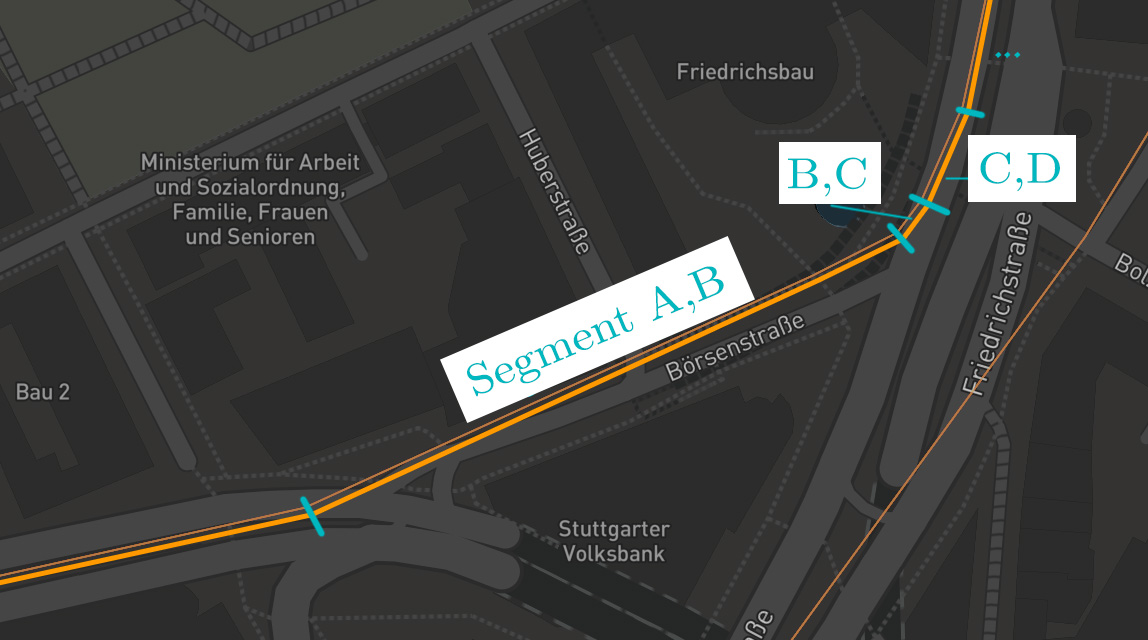
\includegraphics[width=0.45\textwidth]{polyline_segments}
        \caption{Polyline Segmente}
        \label{fig:polyline_segments}
      \end{center}
    \end{figure}

    Das bedeutet, dass die Richtung des Vehicles nicht neu berechnet werden muss, solange es diesem Segment folgt. Erst wenn das Vehicle von Segment $A,B$ auf ein neues Segment $B,C$ übergeht, muss die Richtung neu berechnet werden.

    \item \textbf{Aufteilen der Vehicle in zwei Gruppen:} Da der User durch seinen Bildschirm meistens nur einen Teil der Vehicle zu sehen bekommt, sind die Vehicle in die Gruppen unterteilt. Namentlich seien sie als \texttt{Innerhalb} und \texttt{Außerhalb} benannt. Die Gruppe Innerhalb besitzt all diejenigen Vehicle, die sich im Sichtfeld des Anwenders befinden. Diese werden bei der Animation bevorzugt behandelt und erhalten die volle Rechenleistung. Die Gruppe Außerhalb liegt nicht im Sichtfelds und wird maximal jede Sekunde nach ihrer Aktivität geprüft. Dadurch bleibt auch diese Gruppe immer aktuell.    
   
  \end{itemize}

% subsubsection verbesserung_der_client_performance (end)
    \subsubsection{UI Komponenten}
\label{ssub:ui_komponenten}

  In diesem Abschnitt sollen die verschiedenen UI-Komponenten vorgestellt werden.

  \subsubsection*{Die Karte}
  \label{ssub:die_karte}
    Die Karte (\ref{fig:map}) ist standardmäßig auf den Längengrad 9.244 und Breitengrad 48.757 ausgerichtet. Damit findet sich der Anwender beim Aufrufen der Applikation gleich an der richtigen Stelle wieder. Die Karte verwendet eine abgeänderte Version des Kartenstils \texttt{Mapbox-Dark}. Dabei wurden Parks, Grünflächen und Wasser subtil eingefärbt und die Routen des GTFS-Feeds mit einem leichtem Orange hervorgehoben.

    \begin{figure}[htbp]
      \begin{center}
        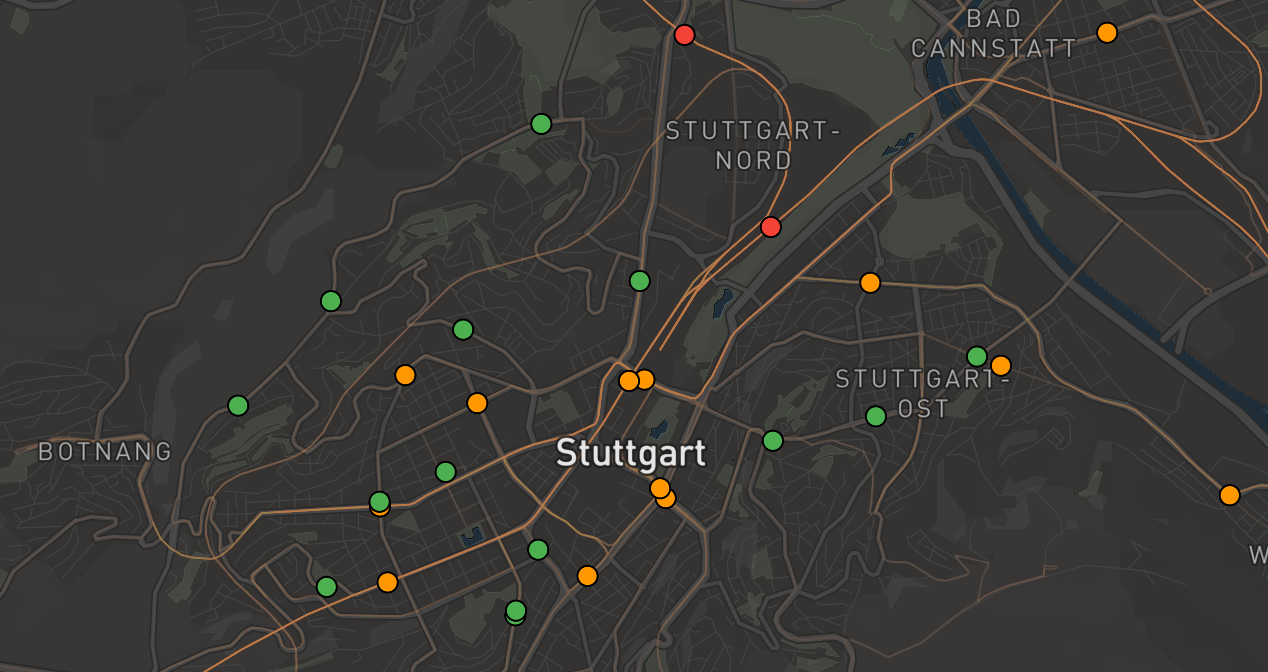
\includegraphics[width=0.6\textwidth]{map}
        \caption{Die Karte mit angepasstem Style: Mapbox-Dark}
        \label{fig:map}
      \end{center}
    \end{figure}
    
  % subsubsection die_karte (end)

  \subsubsection*{Vehicle}
  \label{ssub:vehicle_auf_karte}
    Die Vehicle sind auf der Karte als Kreis dargestellt. Die gegebene Farbe orientiert sich dabei an den öffentlichen Farben des Verkehrsunternehmens. Zum Beispiel sind Interrail Züge im Rot der Deutschen Bahn dargestellt und die U und S-Bahn hat das Orange von Stuttgart-VVS.\\

    Vehicle werden auf der Karte Animiert, wenn sie aktiv. Abbildung \ref{fig:vehicle_states} zeigt die zwei verschiedenen Animationen, die ein Vehicle beim Beginnen und Beendigen des Trips annehmen kann. Wird ein Trip aktiv, so wird das dazugehörende Vehicle auf die Karte platziert. Dabei ist der Radius des Vehicles verringert, bis er der Größe der anderen Vehicle entspricht.

    \begin{figure}[htbp]
      \centering
      \subfloat[Vehicle beginnt seinen Trip und wird aktiv]{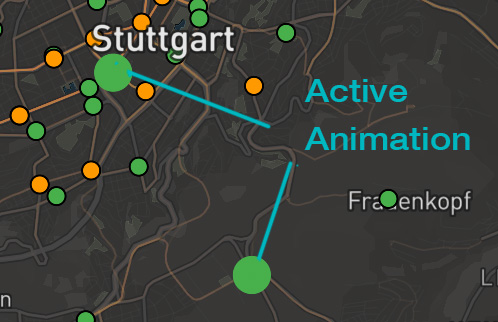
\includegraphics[width=0.34\textwidth]{vehicle_active.jpg}\label{fig:vehicle_active}}
      \hfill
      \subfloat[Vehicle beendet seinen Trip innerhalb von 30 Sekunden und wird inaktiv]{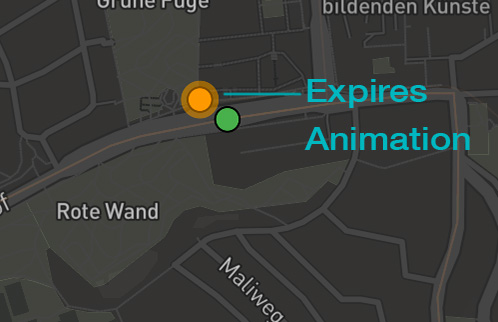
\includegraphics[width=0.34\textwidth]{vehicle_expires.jpg}\label{fig:vehicle_expires}}
      \caption{Vehicle Status Anzeige}
      \label{fig:vehicle_states}
    \end{figure}

    
    Ist ein Vehicle dabei seinen Trip innerhalb von 30 Sekunden zu beenden, so wird ein leicht transparentes Pulsieren angezeigt. Nachdem das Vehicle den Trip beendet hat, wird es von der Karte genommen und verschwindet. Technisch betrachtet werden erst alle Referenzen auf das Vehicle beseitigt und anschließend das Vehicle Objekt gelöscht.
    
  % subsubsection vehicle (end)

  \subsubsection*{Zeitstrahl}
  \label{ssub:zeitstrahl}
    Der Zeitstrahl in Abbildung \ref{fig:timeline} besteht aus mehreren Einzelteilen. 

    \begin{figure}[htbp]
      \begin{center}
        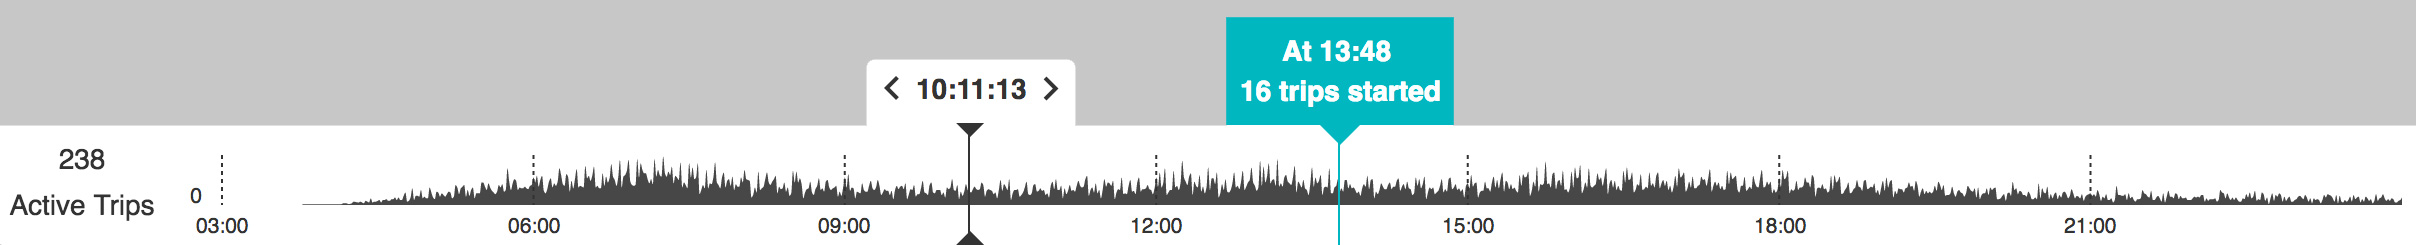
\includegraphics[width=\textwidth]{timeline}
        \caption{Zeitstrahl Komponente}
        \label{fig:timeline}
      \end{center}
    \end{figure}

    Links unten ist die Anzahl an momentan aktiven Trips zu sehen. Diese Anzahl korreliert mit den Vehicles auf der Karte. Die Anzeige wird immer aktuell gehalten und steigt, falls neue Trips aktiv werden, oder fällt wenn ein Trip beendet ist. Der Zeitstrahl selbst zeigt die Anzahl an aktiv werdenden Trips pro Minute an. Bewegt der Anwender die Maus darüber, so bekommt er die genaue Trip Anzahl zu einer Uhrzeit als Tooltip angezeigt. Ebenfalls ist es möglich die Animation zu einem beliebigem Zeitpunkt anzuzeigen. Dafür kann der Anwender einfach auf die gewünschte Zeitmarke im Zeitstrahl klicken und die Animation aktualisiert sich. Damit lässt sich die Karte zu unterschiedlichen Tageszeiten untersuchen. Zuletzt ist auch die gewählte Uhrzeit auf dem Zeitstrahl zu sehen. Diese zeigt dem Anwender, welcher Zeitpunkt momentan auf der Karte angezeigt wird.
    
  % subsubsection zeitstrahl (end)

  \subsubsection*{Filter}
  \label{ssub:filter}
    Über ein ausklappbares Menü, lassen sich verschiedene Filter auswählen. Dadurch kann der Anwender zum Beispiel alle Vehicle eines Typs oder einer Linie darzustellen. Auch Kombinationen der \texttt{Filter Vehicles} und \texttt{Filter Lines} sind möglich. Da aber meist eine Linie von genau einem Vehicle Typ bedient wird, macht das oft keinen Sinn.

    Damit der Anwender die Relation zwischen dem Filter und den Vehicle auf der Karte versteht, sind die Farben einheitlich gestaltet. Nachdem ein Filter ausgewählt ist, kann das Menü entweder wieder zugeklappt werden, oder der Filter lässt sich wieder abwählen.

    \begin{figure}[htbp]
      \begin{center}
        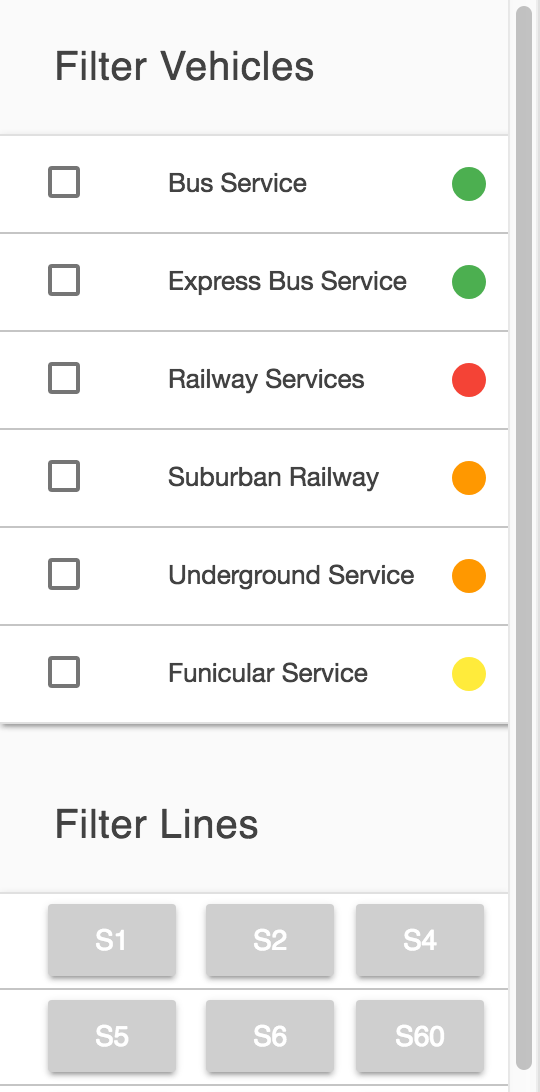
\includegraphics[width=0.2\textwidth]{filter}
        \caption{Filter Funktion}
        \label{fig:filter}
      \end{center}
    \end{figure}
    
  % subsubsection filter (end)

  \subsubsection*{Anzeigen von Trip Informationen}
  \label{ssub:anzeigen_von_trip_informationen}
    Wenn der Anwender ein Vehicle in der Karte durch Klicken auswählt, öffnet sich ein Fenster, welches Informationen für diesen Trip anzeigt (Abbildung \ref{fig:trip_information}. Neben dem Namen der Route lässt sich im Kreis (hier in Rot) die Routen Nummer ablesen. Im unteren Bereich sind die Fahrplaninformationen für den Trip gelistet. Neben dem Namen der Station ist auch die Abfahrtzeit des Vehicles gelistet. Die bereits besuchten Stationen werden in einem Grauton dargestellt um sie als inaktiv zu markieren.


    \begin{figure}[htbp]
      \begin{center}
        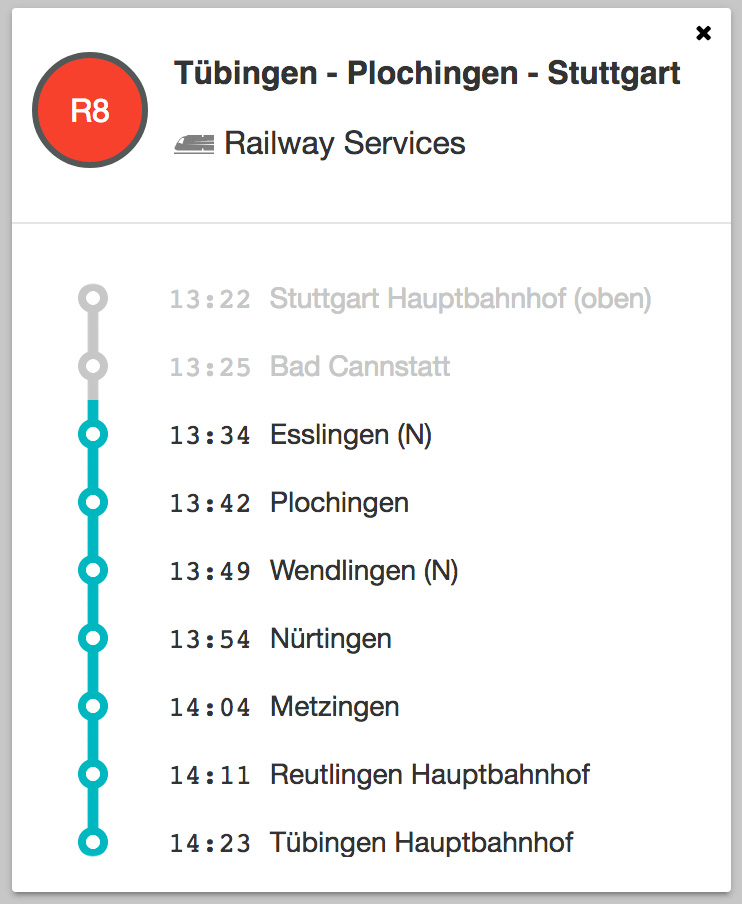
\includegraphics[width=0.3\textwidth]{trip_information}
        \caption{Anzeigen von Trip Informationen}
        \label{fig:trip_information}
      \end{center}
    \end{figure}

    \pagebreak
    
  % subsubsection anzeigen_von_trip_informationen (end)

  \subsubsection*{Wechseln der Kartendarstellung}
  \label{ssub:style_auswahl}
    Über das \texttt{Switch Style} \inlinegraphics{switch_styles_symbol} Element hat der Anwender die Möglichkeit zwischen verschiedenen Darstellungsarten der Karte zu wechseln. Auch die Polylines der Routen lassen sich zusätzlich über das Anwählen von \texttt{Shape} ein- oder ausblenden. Standardmäßig ist \texttt{Dark} ausgewählt.

    \begin{figure}[htbp]
      \begin{center}
        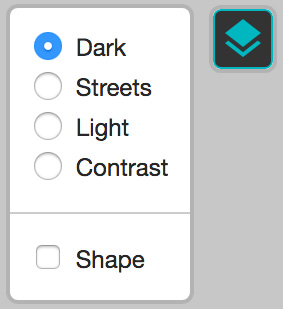
\includegraphics[width=0.14\textwidth]{switch_styles}
        \caption{Wechseln zwischen verschiedenen Kartendarstellung}
        \label{fig:switch_styles}
      \end{center}
    \end{figure}
    
  % subsubsection style_auswahl (end)

  \subsubsection*{Linien Finder}
  \label{ssub:linien_finder}
    Durch klicken des \texttt{Line Finder} \inlinegraphics{line_finder_symbol} Buttons lässt sich auf der Karte eine Route finden, die zwei Stationen $A, B$ verbindet. Dafür setzt der Anwender zwei Pins auf die Karte. Danach sucht ein Algorithmus diejenige Route aus, die am besten diese Stationen verbindet. Das Ergebnis sieht dann wie folgt aus:

    \begin{figure}[htbp]
      \begin{center}
        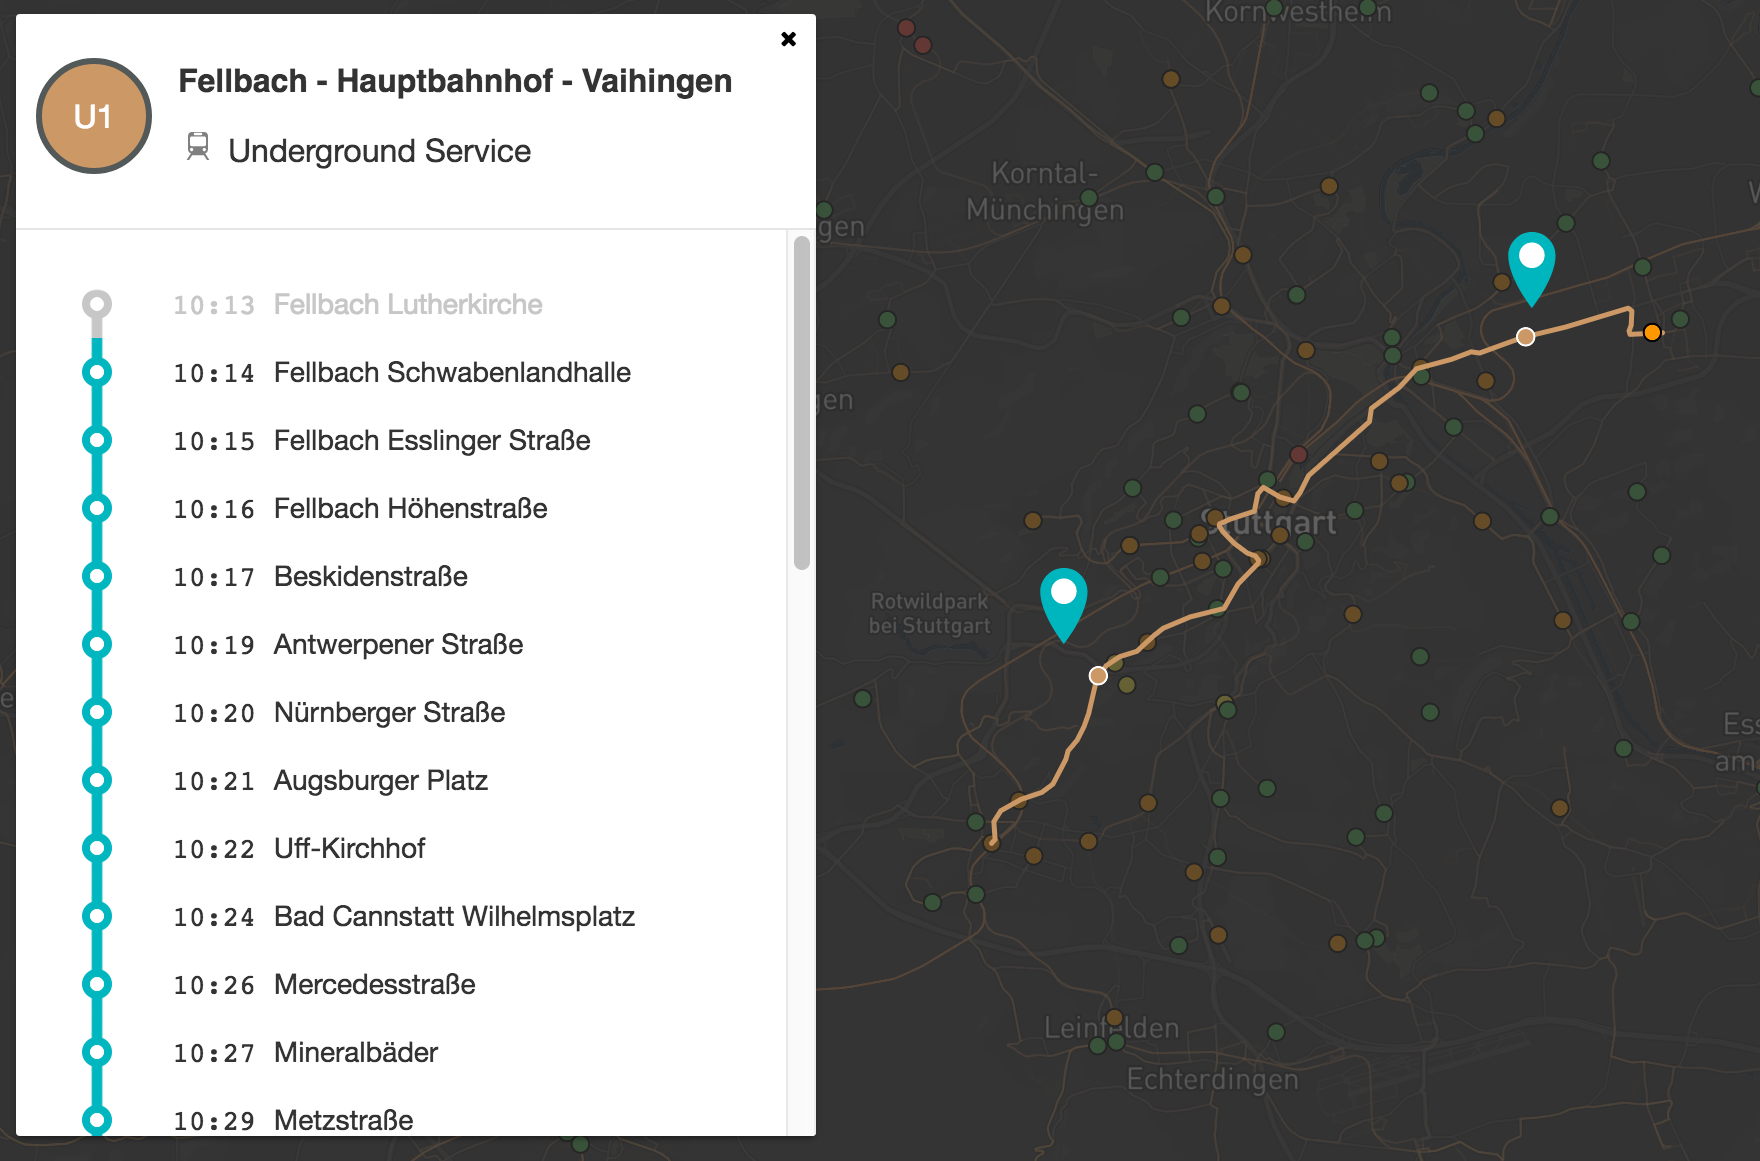
\includegraphics[width=0.6\textwidth]{line_finder}
        \caption{Linien Finder}
        \label{fig:line_finder}
      \end{center}
    \end{figure}

    Diese Funktion vereint Visualisierung und Wegfindung in einer Applikation. Während wir momentan ausschließlich eine Wegfindung über verschiedene Formularfelder (Von..., Nach..., Datum, Uhrzeit) beginnen, könnte es für städtische oder regionale Wegfindung auch eine visuelle Lösung geben. Der Vorteil liegt dabei, dass kein Kontextwechsel nötig ist. Die Orientierung, Wegfindung und Fahrplaninformationen ließen sich alle in einer Ansicht unterbringen. Ein weiteres Merkmal dieses visuellen Ansatzes ist die Möglichkeit eine Route zu finden, ohne dass die Namen der Haltestellen bekannt sein müssen. Das auf der Karte dargestellte Ergebnis, zeigt dem Nutzer auch gleich, wo sich das zur Route gehörende Vehicle sich befindet. Damit könnte der Anwender auch gleich entscheiden, ob er dieses Vehicle noch erreichen würde oder nicht. Dabei ließen sich auch sehr gut GTFS-Realtime Informationen verwenden, so dass man gleich sehen würde ob das Vehicle zum Beispiel Verspätung hat.\\

    Von allen implementierten Komponente hat der Linien Finder am meisten Potential für verschiedene Weiterentwicklungen. Angefangen von der Implementierung von Echtzeitinformationen, über eine integrierte Anwender Navigation (zum Beispiel könnte man den Anwender zu einer Station navigieren), als auch das Anbieten von Möglichkeiten zum Verbindungsanschluss wären möglich. Ebenfalls kann der Algorithmus zur Auswahl der empfohlenen Route noch sehr viel weiter verbessert werden. Momentan fließt vor allem die mittlere Distanz zwischen gesetztem Pin und nächster Station in die Entscheidung ein. Weitere Faktoren könnten aber noch berücksichtigt werden. Beispielsweise der Typ des Vehicles (U-Bahn bevorzugt gegenüber Bus), Frequenz der Route, Wartezeit auf das Vehicle, Preis, Reisezeit oder gar das momentane Verkehrsaufkommen.
    
  % subsubsection linien_finder (end)
  

  % * Timeline Component (Time jump + Trip counter, Trips that get active)
  % * Vehicles, Vehicle States (active, inactive)
  % * Filtering mechanism (Lines / Type)
  % * Layer switcher
  % * Route finder
  % * Bezier Easing 
  
% subsubsection ui_komponenten (end)


  % subsection frontend (end)

\end{newpage}

  % section develop (end)
\end{newpage}